\documentclass[11pt,a4paper]{article}

% ============ PAQUETES EXIGIDOS POR LA GUÍA ============
\usepackage[utf8]{inputenc}
\usepackage[T1]{fontenc}
\usepackage{lmodern}
\usepackage[spanish]{babel}
\usepackage{amsmath}       % ecuaciones (equation, align)
\usepackage{graphicx}      % \includegraphics
\usepackage{booktabs}      % tablas profesionales
\usepackage{siunitx}       % unidades (tiempo en segundos, etc.)
\usepackage{listings}      % código fuente
\usepackage[style=ieee]{biblatex}  % bibliografía estilo IEEE
\usepackage{hyperref}
\usepackage{geometry}
\geometry{margin=2.5cm}

\addbibresource{references_U4.bib}

% Configuración básica de listings para Python
\lstset{
  language=Python,
  basicstyle=\ttfamily\small,
  keywordstyle=\color{blue},
  commentstyle=\color{gray},
  stringstyle=\color{orange},
  breaklines=true,
  frame=single,
  numbers=left,
  numberstyle=\tiny
}

\title{Comprobación experimental de la Ley de Amdahl \\ mediante Apache Spark \\
\large Dominio de referencia: BCEL --- SGA Escuela Provincias Unidas \\
(Microservicio Docente)}

\author{
Keyla Bedón \and Juliana Emanuel \and Harol Vinueza \and Pedro Castro \\
\small Aplicaciones Distribuidas (ISR-701) --- Unidad 4 \\
\small Facultad de Ciencias de la Computación --- Universidad Técnica Estatal de Quevedo \\
\small Código de actividad: GA-SUM-05 / PE-U4 --- Período académico 2026--2027 PPA
}
\date{\today}

\begin{document}

\maketitle

% ======================================================
% RESUMEN
% ======================================================
\begin{abstract}
% TODO (Keyla): resumen de ~150-200 palabras. Debe cubrir: objetivo del
% experimento, dominio de referencia (BCEL, microservicio Docente),
% dataset usado (OULAD), metodología (pandas vs PySpark, 5 transformaciones),
% y el hallazgo principal (fracción serial observada, speedup obtenido).
\end{abstract}

\tableofcontents
\newpage

% ======================================================
% 1. INTRODUCCIÓN
% ======================================================
\section{Introducción}
% TODO (Keyla): contexto general -- por qué el procesamiento distribuido
% importa, qué es la Ley de Amdahl en una frase, y cómo se conecta con
% el dominio BCEL (microservicio Docente). Referenciar la sección de
% Fundamento Teórico y de Procedimiento que siguen.

% ======================================================
% 2. FUNDAMENTO TEÓRICO (Sección 5 de la guía)
% ======================================================
\section{Fundamento teórico}

\subsection{Fundamentos de paralelismo y Ley de Amdahl}
\label{sec:amdahl}
% TODO (Juliana) -- Commit 1
% Mínimo 300 palabras. Ver Guia_Juliana.md para el contenido completo
% y las ecuaciones numeradas listas para copiar.

\subsection{Paradigma MapReduce y Apache Hadoop}
\label{sec:mapreduce}
% TODO (Juliana) -- Commit 2
% Mínimo 300 palabras. Ver Guia_Juliana.md.

\subsection{Apache Spark: arquitectura y modelo de programación}
\label{sec:spark}

Apache Spark es un motor de procesamiento distribuido en memoria diseñado para
superar las limitaciones de MapReduce en cargas de trabajo iterativas
\cite{zaharia2012}. Su arquitectura se organiza en tres componentes principales:
el \textit{driver}, proceso que ejecuta la función \texttt{main} de la
aplicación, construye el grafo de operaciones y coordina el trabajo; el
\textit{cluster manager} (YARN, Kubernetes o el gestor \textit{standalone} de
Spark), responsable de asignar recursos físicos a la aplicación; y los
\textit{executors}, procesos distribuidos en los nodos del clúster que ejecutan
las tareas y almacenan los datos en memoria o disco según se requiera
\cite{chambers2018}.

El modelo de datos fundamental de Spark es el RDD (\textit{Resilient
Distributed Dataset}), una colección inmutable y particionada de objetos que
se distribuye entre los nodos del clúster. La tolerancia a fallos de los RDD no
se basa en replicación física de los datos, sino en el \textit{lineage}: cada
RDD conserva el registro de las transformaciones que lo generaron a partir de
su fuente original, de modo que, si una partición se pierde por la falla de un
nodo, Spark puede reconstruirla recalculando únicamente esa porción del linaje,
sin necesidad de releer todo el conjunto de datos desde el almacenamiento
estable \cite{zaharia2012}. Sobre los RDD se construyó posteriormente la API de
\textit{DataFrames} y \textit{Datasets}, que añade un esquema tabular explícito
y permite que el optimizador Catalyst reorganice las operaciones antes de
ejecutarlas \cite{armbrust2015}; esta es la razón por la cual las
transformaciones sobre un DataFrame no se ejecutan necesariamente en el orden
exacto en que se escriben en el código.

Spark distingue entre \textit{transformaciones} (operaciones como
\texttt{filter}, \texttt{groupBy} o \texttt{join}, que son perezosas y solo
construyen un plan lógico) y \textit{acciones} (como \texttt{count} o
\texttt{collect}, que disparan la ejecución real). Esta evaluación perezosa
permite que el motor optimice el plan completo antes de correrlo, en lugar de
ejecutar cada paso de forma aislada. Al invocarse una acción, Spark traduce el
plan lógico en un DAG (grafo acíclico dirigido) de \textit{stages}, cada uno
compuesto por \textit{tasks} que se ejecutan en paralelo sobre las particiones
de datos; los límites entre stages están marcados por operaciones de
\textit{shuffle}, como las requeridas en un \texttt{join} o un
\texttt{groupBy} con reparto de claves \cite{chambers2018}.

Frente a MapReduce, Spark evita escribir los resultados intermedios a disco
entre cada fase, manteniéndolos en memoria siempre que es posible, lo que
reduce drásticamente la latencia en algoritmos que iteran múltiples veces
sobre el mismo conjunto de datos \cite{zaharia2012}. En el contexto del
dominio BCEL, esta arquitectura resulta directamente aplicable al
procesamiento del histórico de asistencias y calificaciones del microservicio
Docente: operaciones como el \texttt{join} entre la tabla de calificaciones y
la de matrículas (T3 de esta práctica) se benefician tanto del particionamiento
distribuido de los DataFrames como de la posibilidad de reejecutar únicamente
las tareas afectadas ante un fallo parcial del clúster, sin reprocesar el
conjunto completo.

\subsection{Computación en la nube: modelos y proveedores}
\label{sec:cloud}

El Instituto Nacional de Estándares y Tecnología de Estados Unidos (NIST)
define la computación en la nube como un modelo que permite acceso ubicuo,
conveniente y bajo demanda a un conjunto compartido de recursos informáticos
configurables (redes, servidores, almacenamiento, aplicaciones y servicios),
que pueden aprovisionarse y liberarse con un esfuerzo mínimo de gestión o de
interacción con el proveedor \cite{mell2011}. Esta definición identifica cinco
características esenciales: autoservicio bajo demanda, donde el usuario
aprovisiona recursos sin intervención humana del proveedor; acceso amplio a
la red, disponible desde plataformas heterogéneas; \textit{pooling} de
recursos, que multiplexa capacidad física entre varios consumidores mediante
un modelo multiusuario; elasticidad rápida, que permite escalar recursos casi
instantáneamente según la demanda; y servicio medido, donde el consumo se
monitorea y factura de forma transparente \cite{mell2011}.

Sobre esa base, el NIST distingue tres modelos de servicio, a los que la
industria ha añadido un cuarto: \textit{Infrastructure as a Service} (IaaS),
donde el proveedor entrega recursos de cómputo, almacenamiento y red en bruto,
y el cliente gestiona el sistema operativo y las aplicaciones; \textit{Platform
as a Service} (PaaS), que añade un entorno de ejecución gestionado sobre el
cual el cliente despliega su código sin administrar la infraestructura
subyacente; \textit{Software as a Service} (SaaS), donde el cliente consume
una aplicación completa gestionada íntegramente por el proveedor; y
\textit{Function as a Service} (FaaS), un modelo de cómputo sin servidor donde
el proveedor ejecuta funciones individuales en respuesta a eventos, facturando
únicamente por el tiempo de ejecución real \cite{burns2024}.

Para el procesamiento distribuido de datos, los tres proveedores dominantes
ofrecen servicios administrados equivalentes que abstraen la gestión manual
del clúster: Amazon EMR (\textit{Elastic MapReduce}) en AWS, Azure HDInsight
en Microsoft Azure, y Google Cloud Dataproc en GCP. Los tres permiten
aprovisionar clústeres de Spark y Hadoop bajo demanda, integrarse con el
almacenamiento de objetos del proveedor (S3, Blob Storage o Cloud Storage,
respectivamente) y escalar el número de nodos según la carga, delegando en el
proveedor tareas como el parcheo del sistema operativo o la configuración de
red del clúster \cite{burns2024}.

Finalmente, cuando el procesamiento por lotes debe combinarse con datos que
llegan en tiempo real, surgen dos patrones arquitectónicos complementarios.
La arquitectura Lambda mantiene dos rutas de procesamiento paralelas: una capa
por lotes que recalcula vistas completas sobre el histórico con alta
precisión, y una capa de velocidad que procesa el flujo reciente con baja
latencia para cubrir el retraso de la capa por lotes, fusionando ambas en una
capa de servicio. La arquitectura Kappa simplifica este esquema eliminando la
capa por lotes: todo el procesamiento, tanto histórico como en tiempo real, se
ejecuta sobre un único motor de streaming, reprocesando el flujo completo
desde el log de eventos cuando se requiere recalcular una vista
\cite{burns2024}. En el dominio BCEL, el microservicio Docente ya opera sobre
AWS EC2 con PostgreSQL; si el volumen de asistencias y calificaciones
creciera hasta justificar un motor distribuido de forma sostenida, la
migración natural sería hacia Amazon EMR, evitando la gestión manual de un
clúster Spark autoadministrado y aprovechando la integración directa con el
resto de servicios AWS ya utilizados por el sistema.


% ======================================================
% 3. PROCEDIMIENTO APLICADO (Sección 7 de la guía, narrado)
% ======================================================
\section{Procedimiento aplicado}
% TODO (Keyla) -- Commit 3
% Narrar en prosa (no solo pegar código) los Pasos 1-4 realmente
% ejecutados en el notebook: preparación del entorno y dataset,
% implementación pandas, implementación PySpark (incluir aquí la
% configuración efectiva de Spark obtenida con
% spark.sparkContext.getConf().getAll()), y protocolo de medición.

\subsection{Entorno y conjunto de datos}
% TODO (Keyla): tabla booktabs con fuente/URL/licencia/fecha/registros
% (copiar de data/README_dataset.md)

\subsection{Evidencia de ejecución: Spark UI}
% TODO (Keyla): insertar aquí la captura de evidencia/spark_ui_t3.png
\begin{figure}[h]
  \centering
  % \includegraphics[width=0.9\textwidth]{../evidencia/spark_ui_t3.png}
  \caption{DAG y stages del job de T3 (join) en la interfaz de Spark (Spark UI)}
  \label{fig:spark_ui}
\end{figure}
% No olvidar referenciar esta figura desde el texto con \ref{fig:spark_ui}

% ======================================================
% 4. RESULTADOS (Sección 2.3/2.4 de la rúbrica)
% ======================================================
\section{Resultados}

\subsection{Tiempos de ejecución}
% TODO (Pedro) -- Commit 1
% Tabla booktabs + siunitx con tiempos pandas vs pyspark por transformación.
% Ejemplo de estructura:
%
% \begin{table}[h]
% \centering
% \begin{tabular}{lS[table-format=2.4]S[table-format=2.4]S[table-format=1.3]}
% \toprule
% {Transformación} & {pandas (\si{\second})} & {PySpark (\si{\second})} & {Speedup} \\
% \midrule
% T1 & ... & ... & ... \\
% T2 & ... & ... & ... \\
% T3 & ... & ... & ... \\
% T4 & ... & ... & ... \\
% T5 & ... & ... & ... \\
% \bottomrule
% \end{tabular}
% \caption{Tiempos medianos de ejecución (pandas vs. PySpark) por transformación}
% \label{tab:tiempos}
% \end{table}

\subsection{Figuras}
% TODO (Pedro) -- Commit 1
% Insertar las 3 figuras generadas por src/graficas.py, con \caption,
% \label, y un párrafo de interpretación propio de cada una.

\begin{figure}[h]
  \centering
  % 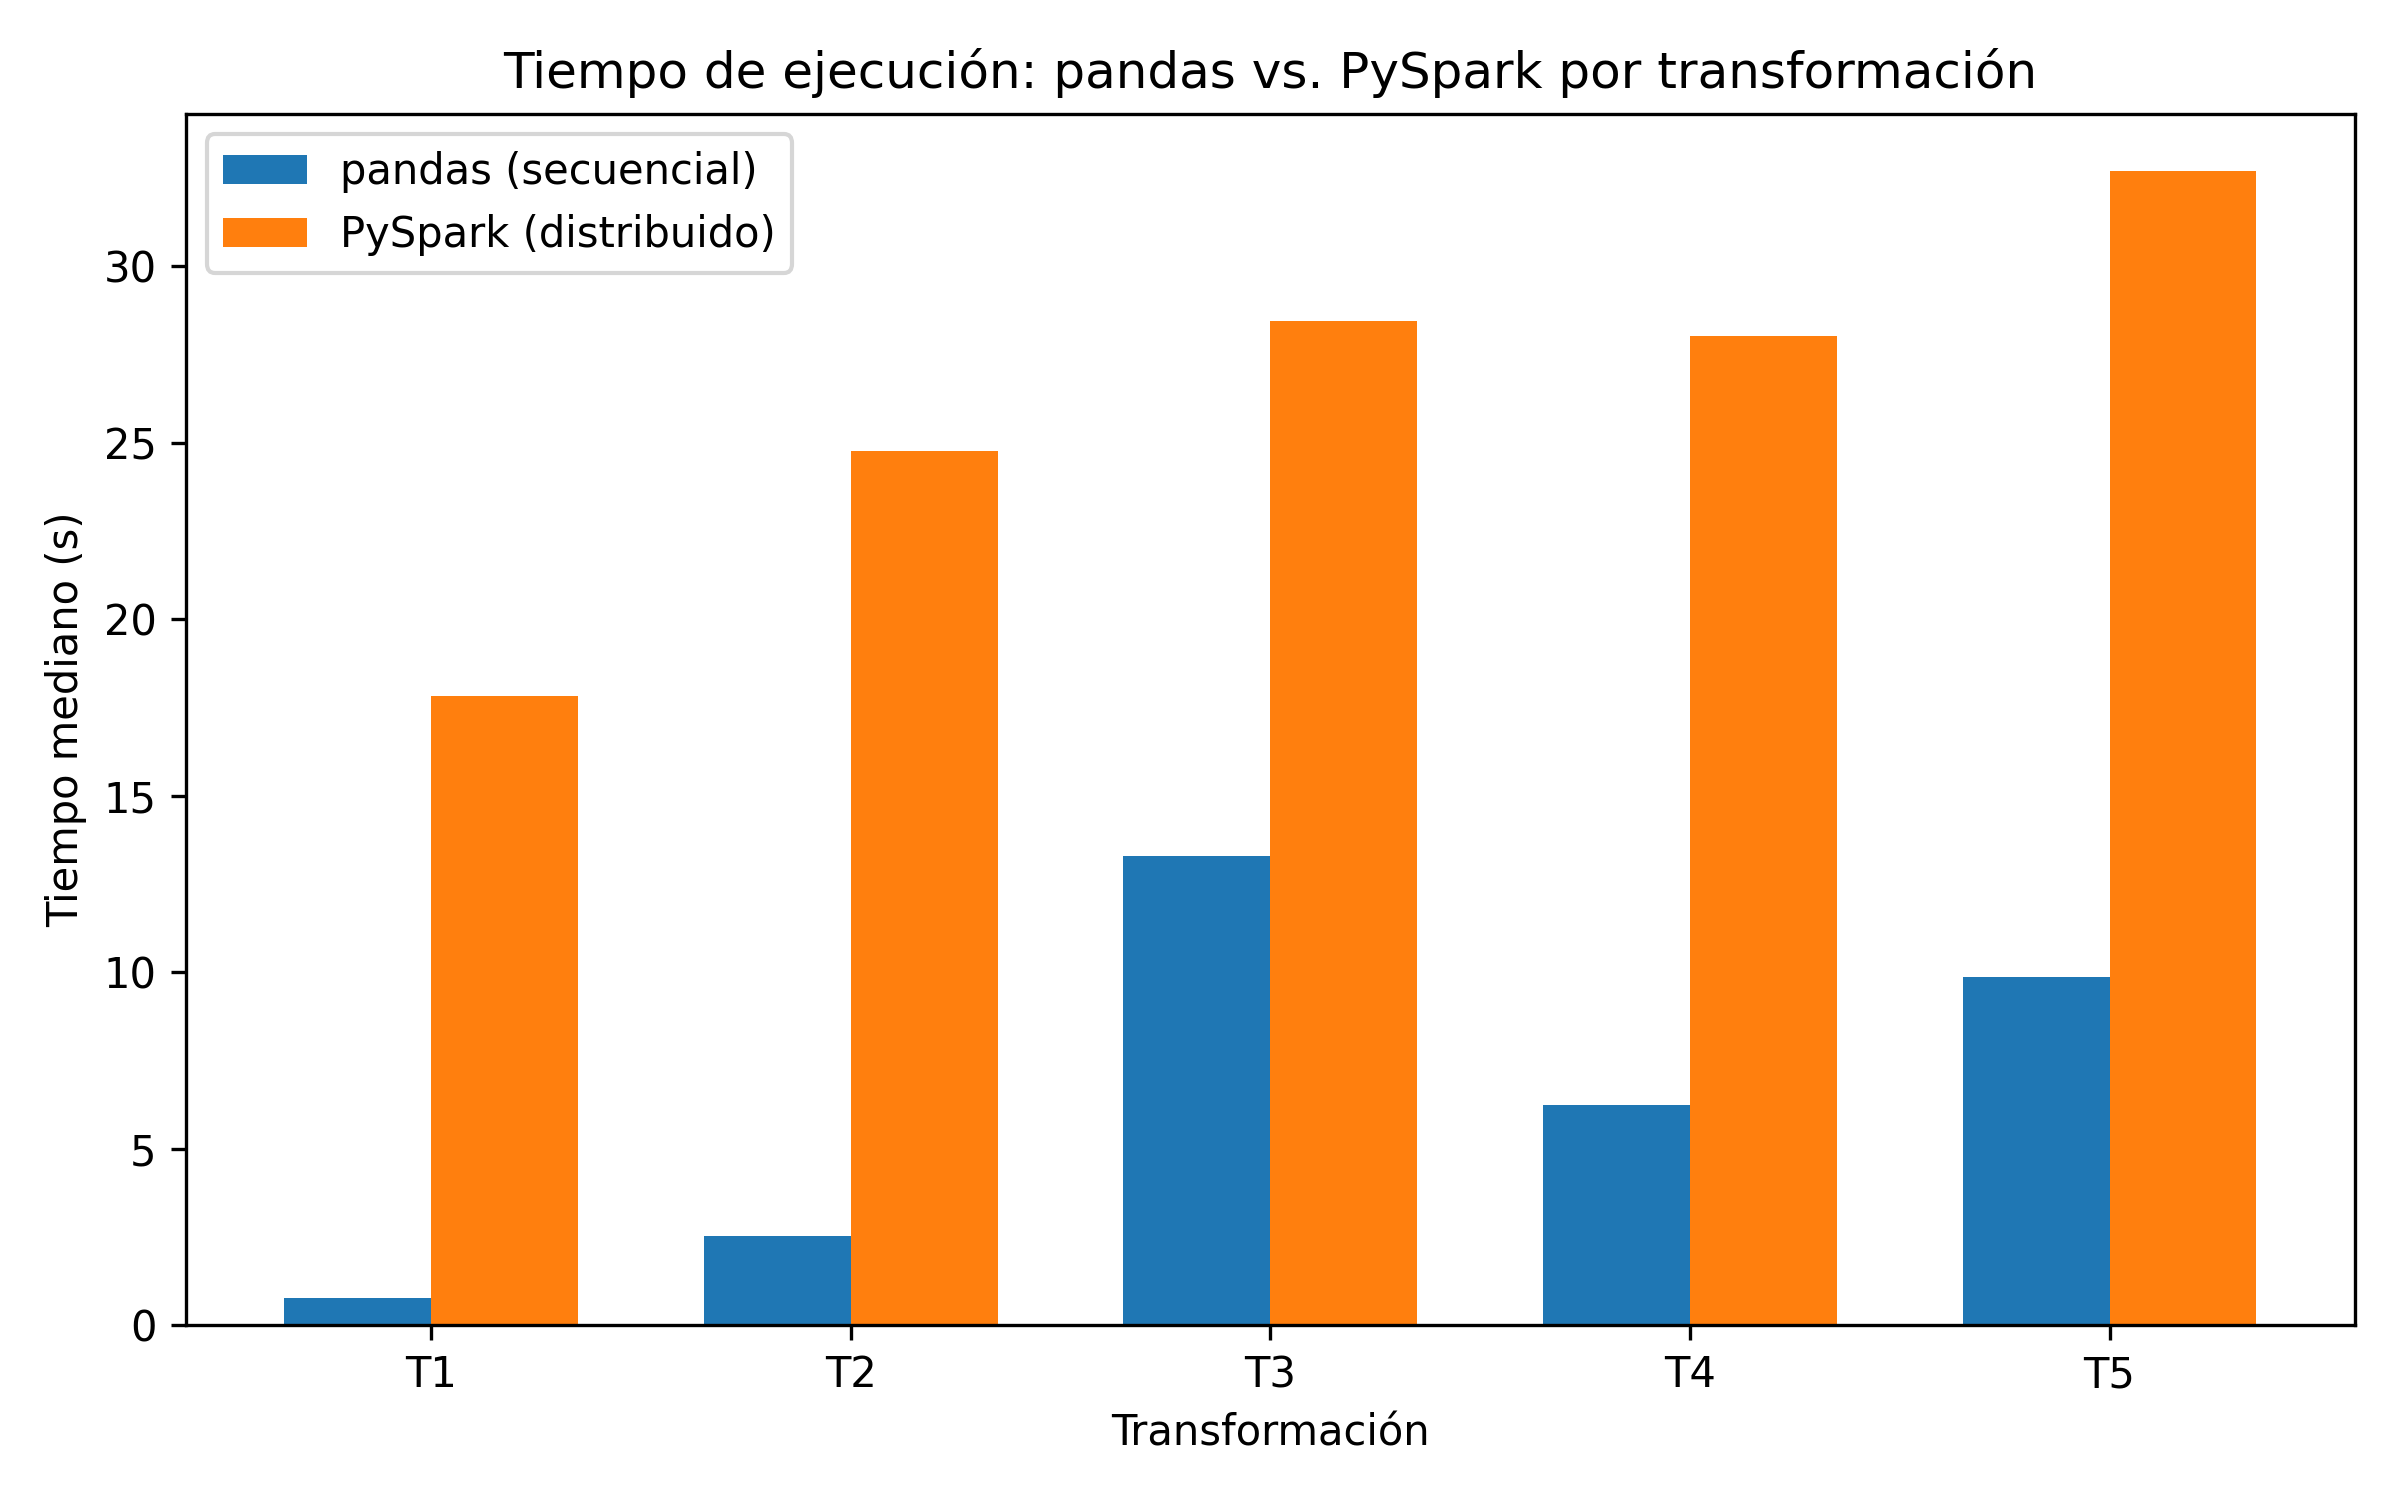
\includegraphics[width=0.8\textwidth]{../resultados/figuras/fig1_barras.png}
  \caption{Tiempo de ejecución: pandas vs. PySpark por transformación}
  \label{fig:barras}
\end{figure}
% Interpretación de la Figura \ref{fig:barras}: ...

\begin{figure}[h]
  \centering
  % 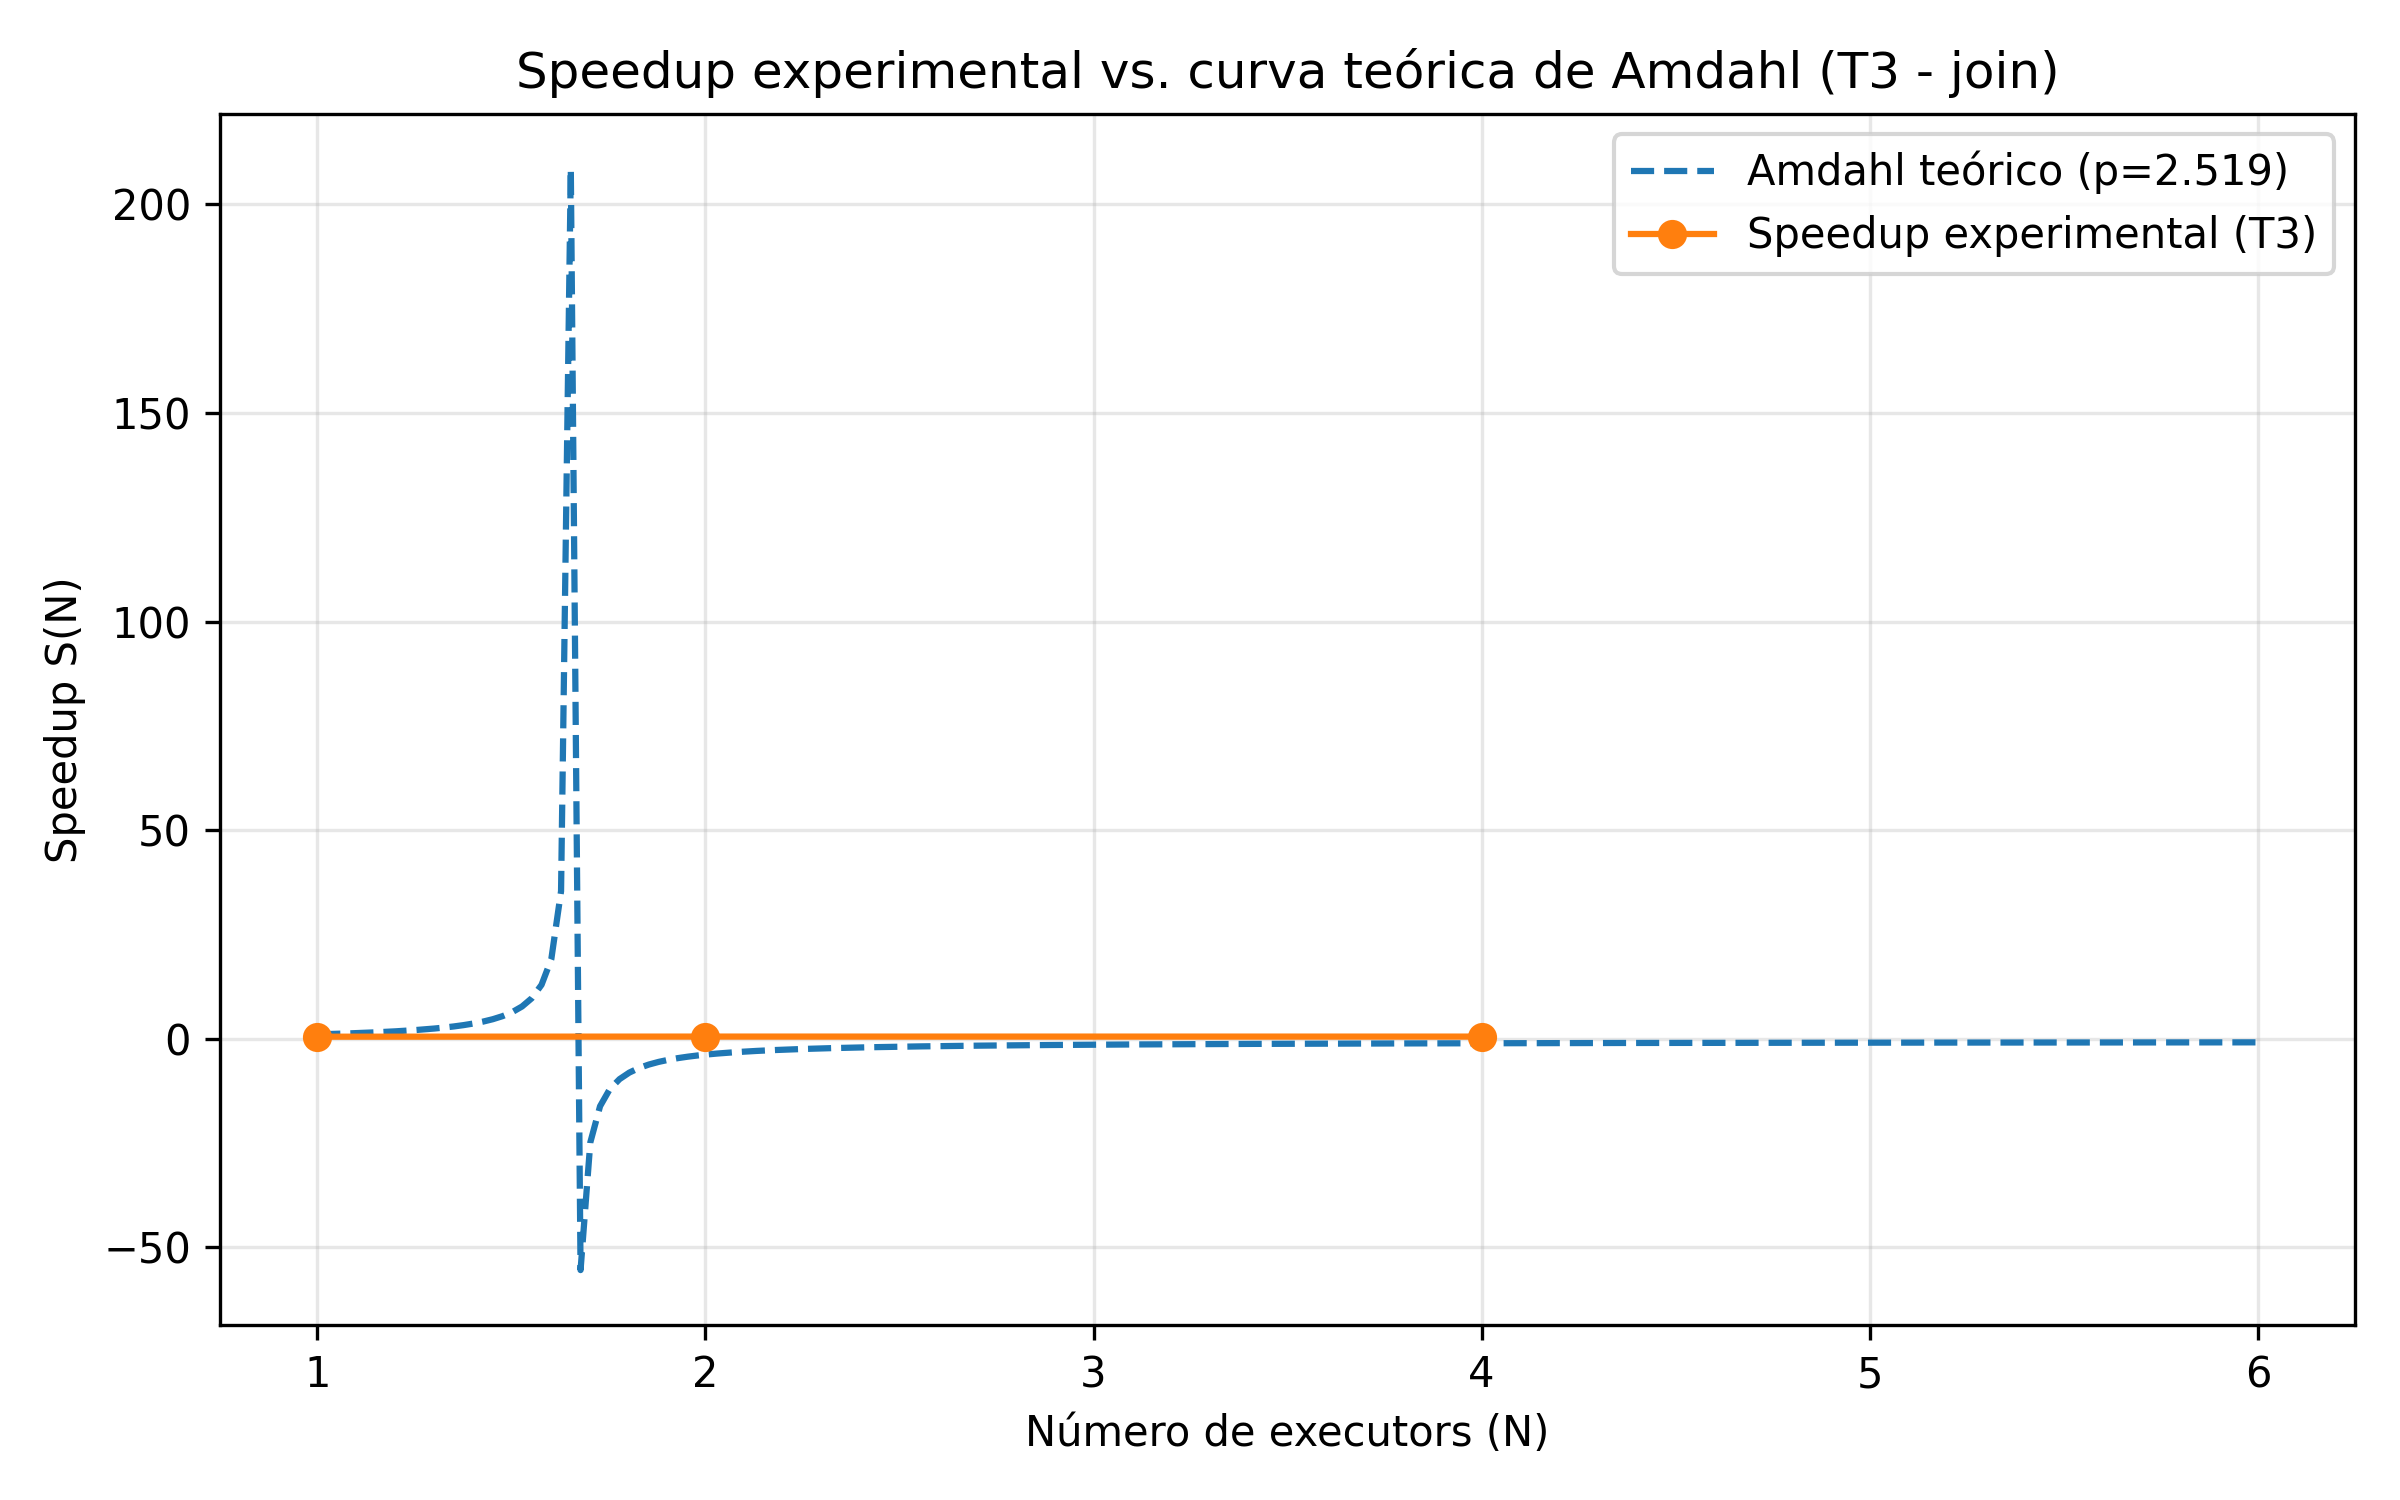
\includegraphics[width=0.8\textwidth]{../resultados/figuras/fig2_speedup.png}
  \caption{Speedup experimental vs. curva teórica de Amdahl (T3 - join)}
  \label{fig:speedup}
\end{figure}
% Interpretación de la Figura \ref{fig:speedup}: ...

\begin{figure}[h]
  \centering
  % 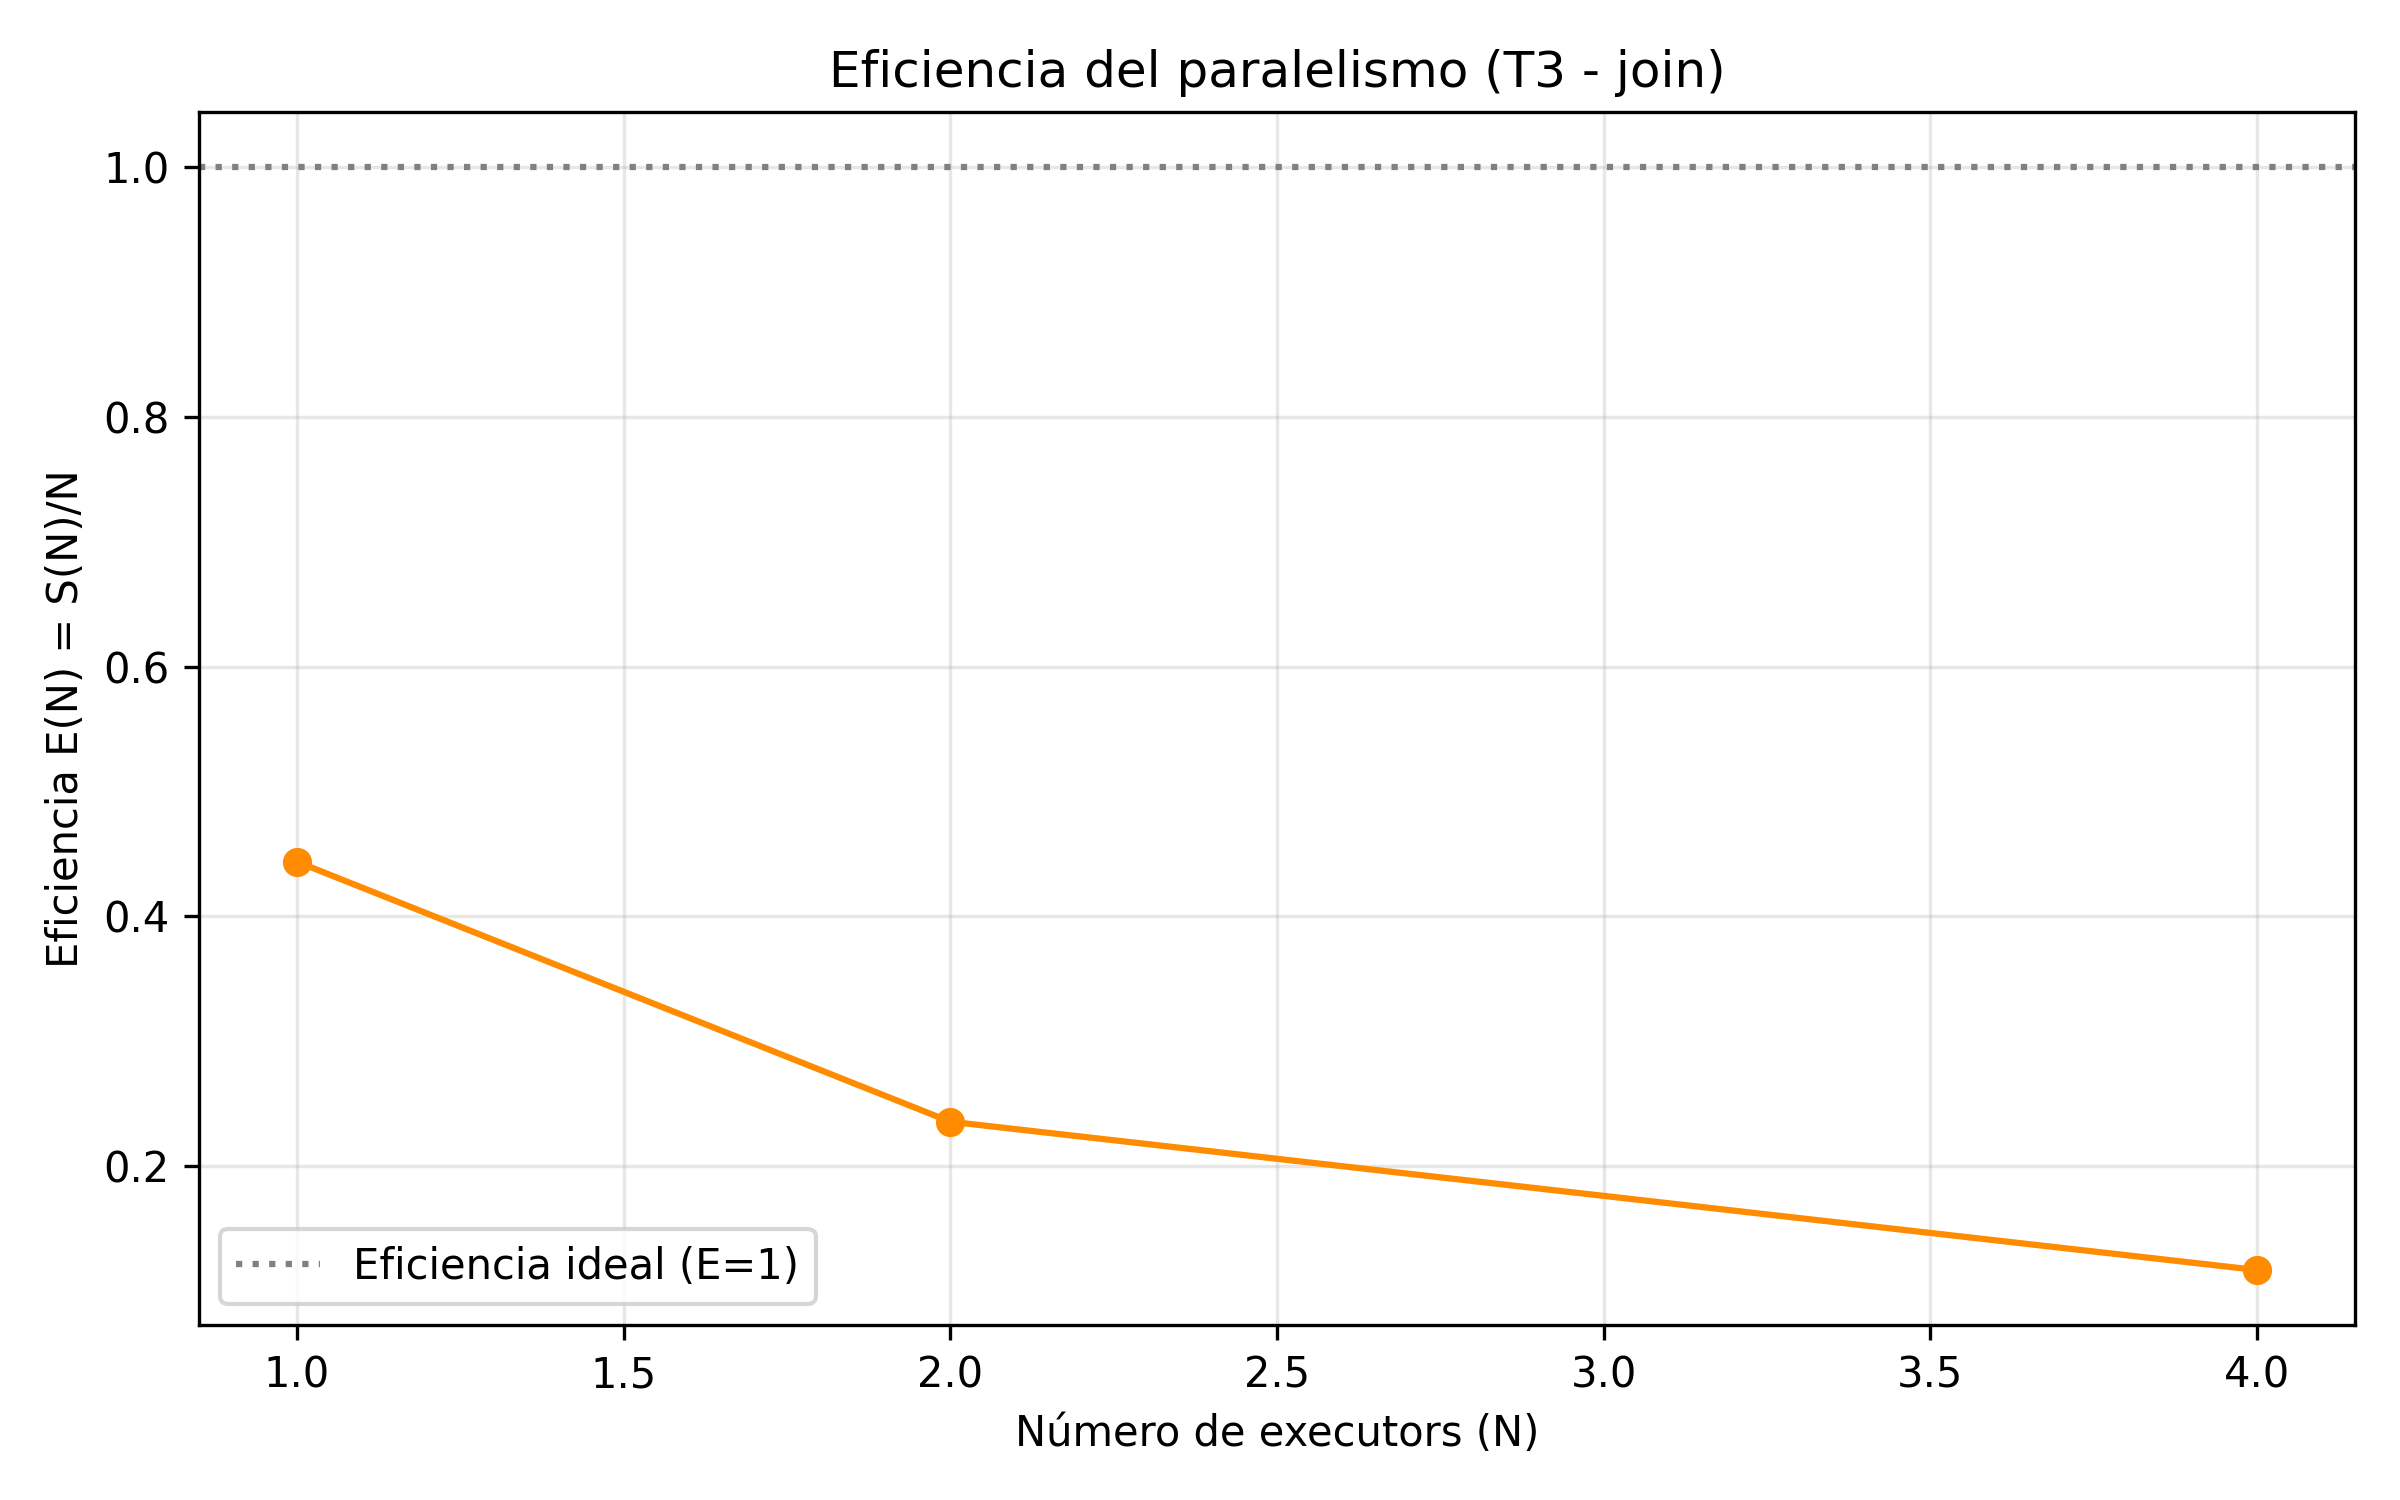
\includegraphics[width=0.8\textwidth]{../resultados/figuras/fig3_eficiencia.png}
  \caption{Eficiencia del paralelismo E(N) = S(N)/N (T3 - join)}
  \label{fig:eficiencia}
\end{figure}
% Interpretación de la Figura \ref{fig:eficiencia}: ...

% ======================================================
% 5. ANÁLISIS CRÍTICO
% ======================================================
\section{Análisis crítico}
% TODO (todo el equipo): discutir el umbral de volumen de datos a partir
% del cual Spark resulta rentable frente a pandas en el dominio BCEL,
% conectando con las preguntas del Anexo A.

% ======================================================
% 6. PREGUNTAS DE ANÁLISIS (Anexo A)
% ======================================================
\section{Preguntas de análisis}

\subsection*{Pregunta 1}
% TODO (Keyla) -- Commit 3. Mínimo 200 palabras.

\subsection*{Pregunta 2}
% TODO (Pedro) -- Commit 2. Mínimo 200 palabras.

\subsection*{Pregunta 3}
% TODO (Juliana) -- Commit 2. Mínimo 200 palabras.

\subsection*{Pregunta 4}

Spark supera a MapReduce en cargas de trabajo iterativas principalmente por
dos decisiones de diseño: el modelo de \textit{lineage} de los RDD y la
evaluación perezosa. MapReduce materializa el resultado de cada fase Map y
Reduce escribiéndolo en el sistema de archivos distribuido (HDFS) antes de
iniciar la siguiente fase. En un algoritmo iterativo, como los usados en
aprendizaje automático o en el cálculo de PageRank, esto obliga a leer y
escribir el mismo conjunto de datos desde disco en cada iteración, generando
una sobrecarga de E/S que domina el tiempo total de ejecución y que crece
linealmente con el número de iteraciones \cite{zaharia2012}.

Spark evita este cuello de botella manteniendo los datos en memoria entre
operaciones sucesivas mediante los RDD. La tolerancia a fallos de este
modelo no depende de replicar físicamente los datos en disco, sino del
\textit{lineage}: cada RDD conserva el grafo de transformaciones que lo
originó a partir de la fuente de datos. Si un executor falla y se pierde una
partición, Spark no necesita releer todo el conjunto de datos desde el
almacenamiento estable; simplemente recalcula, a partir del lineage, solo la
porción perdida, lo cual resulta considerablemente más barato que la
tolerancia a fallos basada en replicación de MapReduce \cite{zaharia2012}.
Esto permite que un algoritmo iterativo reutilice el mismo RDD en memoria a
través de sucesivas iteraciones sin pagar el costo de E/S en cada una.

La evaluación perezosa complementa esta ventaja desde el plano de la
planificación. Spark no ejecuta las transformaciones (\texttt{map},
\texttt{filter}, \texttt{join}, etc.) en el momento en que se declaran en el
código; en su lugar, construye un plan lógico que solo se materializa cuando
se invoca una acción (\texttt{count}, \texttt{collect}, \texttt{saveAsTextFile}).
Esto le permite al motor observar la cadena completa de operaciones antes de
ejecutar nada, y optimizarla como un todo: puede fusionar transformaciones
consecutivas en una sola pasada sobre los datos, eliminar cómputo redundante
y decidir el punto óptimo para persistir en memoria un RDD que se reutilizará
en varias iteraciones, en lugar de ejecutar cada operación de forma aislada e
inmediata como ocurre en el modelo rígido de fases de MapReduce
\cite{zaharia2016}.

En conjunto, ambos mecanismos explican por qué Spark reporta mejoras de
rendimiento de un orden de magnitud o más frente a MapReduce en cargas
iterativas: el lineage reduce el costo de la tolerancia a fallos sin recurrir
a E/S constante, y la evaluación perezosa permite optimizar globalmente el
plan de ejecución en lugar de ejecutar operación por operación
\cite{zaharia2016}.

% ======================================================
% 7. CONCLUSIONES INDIVIDUALES
% ======================================================
\section{Conclusiones individuales}

\subsection*{Keyla Bedón}
% TODO: mínimo 150 palabras.

\subsection*{Juliana Emanuel}
% TODO: mínimo 150 palabras.

\subsection*{Harol Vinueza}

Esta práctica me permitió comprender de forma concreta por qué Apache Spark
se convirtió en el estándar de facto para el procesamiento distribuido de
datos, más allá de la definición abstracta que suele darse en clase. Trabajar
la arquitectura de Spark en profundidad --- el rol del driver, el cluster
manager y los executors, y sobre todo el mecanismo de lineage de los RDD ---
me hizo entender que la tolerancia a fallos y el rendimiento no son
propiedades independientes: el diseño que permite reconstruir datos perdidos
sin releer todo el dataset es el mismo que permite mantener resultados
intermedios en memoria y evitar la sobrecarga de E/S que castiga a MapReduce
en cargas iterativas. Profundizar en la evaluación perezosa y en cómo el
optimizador Catalyst reordena las operaciones también me cambió la forma en
que voy a escribir código con DataFrames de aquí en adelante, sabiendo que el
orden en que escribo las transformaciones no necesariamente es el orden en
que se ejecutan.

Trabajar la sección de computación en la nube, en particular la comparación
entre EMR, HDInsight y Dataproc, me hizo ver con claridad la ruta de
crecimiento natural para un sistema como BCEL: hoy el microservicio Docente
corre sobre una instancia EC2 con PostgreSQL, una arquitectura suficiente
para el volumen actual, pero que tendría un techo claro si el número de
períodos académicos y estudiantes históricos creciera de forma sostenida. Ver
en la práctica, con el dataset OULAD, cómo cambia el tiempo de ejecución
entre pandas y PySpark según el tamaño y el tipo de operación, me deja una
intuición mucho más sólida sobre cuándo migrar de un procesamiento síncrono y
centralizado a un motor distribuido realmente vale la sobrecarga que implica
adoptarlo.

\subsection*{Pedro Castro}
% TODO: mínimo 150 palabras.

% ======================================================
% 8. DECLARACIÓN DE USO DE IA GENERATIVA
% ======================================================
\section{Declaración de uso de inteligencia artificial generativa}
% TODO (Keyla, con aporte de todos): completar conforme a los
% lineamientos de la asignatura -- herramienta, propósito y secciones
% en las que se usó. Ser honestos y específicos.

% ======================================================
% BIBLIOGRAFÍA
% ======================================================
\newpage
\printbibliography

\end{document}
